\documentclass[12pt]{article}
\usepackage[russian]{babel}
\usepackage[utf8]{inputenc}
\usepackage{amssymb}
\usepackage{mathtools}
\usepackage{mathrsfs}
\usepackage{graphicx}
\usepackage{float}
\usepackage{caption}
\textheight=235mm \textwidth=170mm \hoffset=-20mm \voffset=-20mm

\begin{document}
	\topskip=0mm
	\vspace*{6cm}
	\begin{center}
		\textbf{\Large {\underline{Отчет по лабораторной работе}}}
		\textbf{\Large {\underline{На тему: «Определение свойств канала передачи данных»}}}
	\end{center}
	
	\vspace*{80mm}
	
	\flushleft{\underline{Выполнил}:} \hspace{70mm} {Дробышев Андрей Валентинович}
	\flushleft{\underline{Проверил}:} \hspace{73mm} {Бондаренко Алексей Алексеевич}
	
	\vspace*{\fill} 
	\begin{center}
		Москва 2016
	\end{center}	
	\newpage
	
	\underline{Цель работы}: Определение условий эффективной передачи информации между процессами параллельного
приложения. \\ \medskip 
	\underline{Краткое описание}:\\
		\qquad В данной работе при помощи непосредственных измерений были определены основные характеристики вычислительной сети. \\ \medskip
	\underline{Результаты эксперимента}:\\
		\qquad Были проведены измерения латентности и пропускной способности ("точка-точка" и двунаправленный обмен) в зависимости от длины передаваемого сообщения (length=$2^{k}$ байт, где $k=0, 1, ..., 22$.)\\ \bigskip
		
	Ниже приведены соответствующие графики.
	\begin{figure}[H]
		\centering
		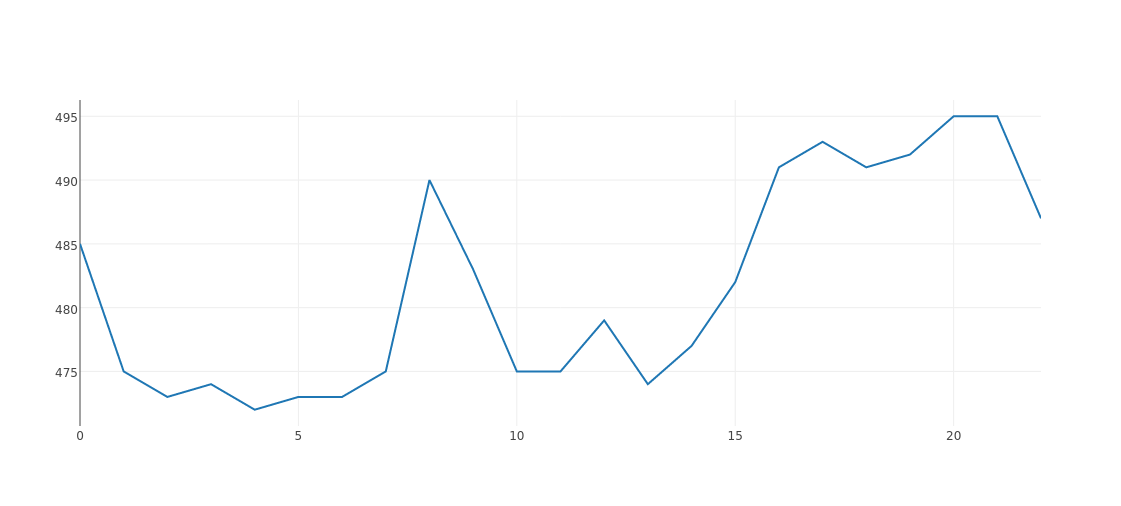
\includegraphics[scale=0.4]{./graphs/lat_int.png}
		\caption{График зависимости s(k), nsec (процессы на одном узле сети)}
		\captionsetup{labelformat=empty}
	\end{figure}
	
	\begin{figure}[H]
		\centering
		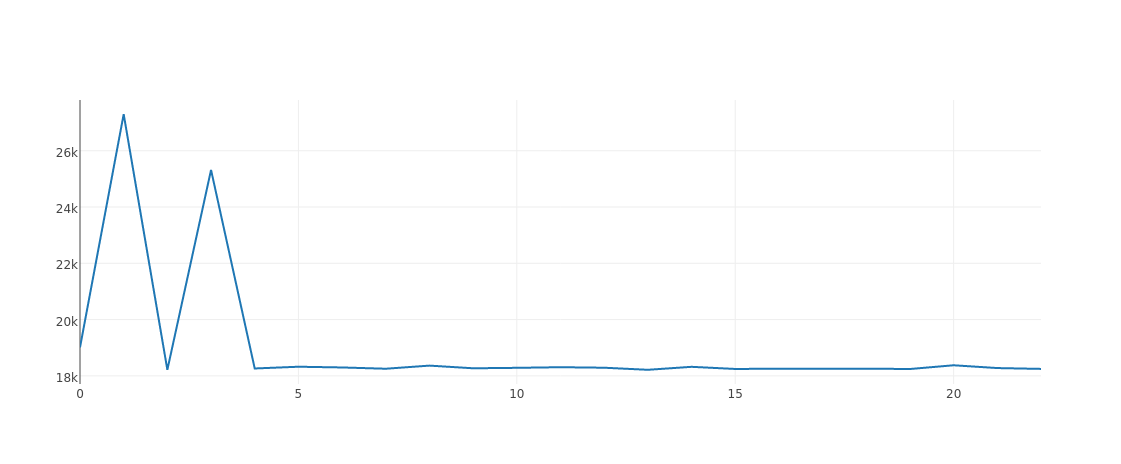
\includegraphics[scale=0.4]{./graphs/lat_ext.png}
		\caption{График зависимости s(k), nsec (процессы на разных узлах сети)}
		\captionsetup{labelformat=empty}
	\end{figure}
	
	\begin{figure}[H]
		\centering
		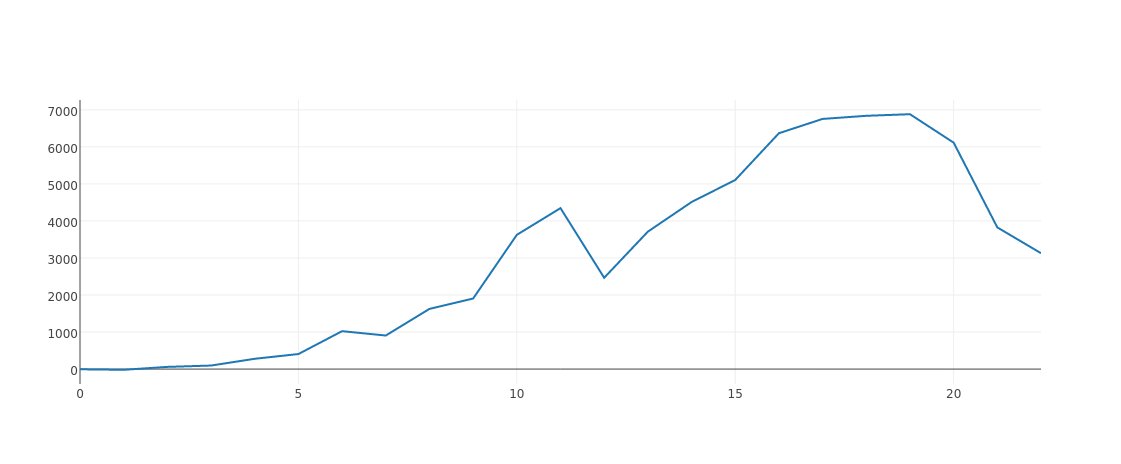
\includegraphics[scale=0.4]{./graphs/ppcap_int.png}
		\caption{График зависимости Rpp(k), Mb/sec (процессы на одном узле сети)}
		\captionsetup{labelformat=empty}
	\end{figure}
	
	\begin{figure}[H]
		\centering
		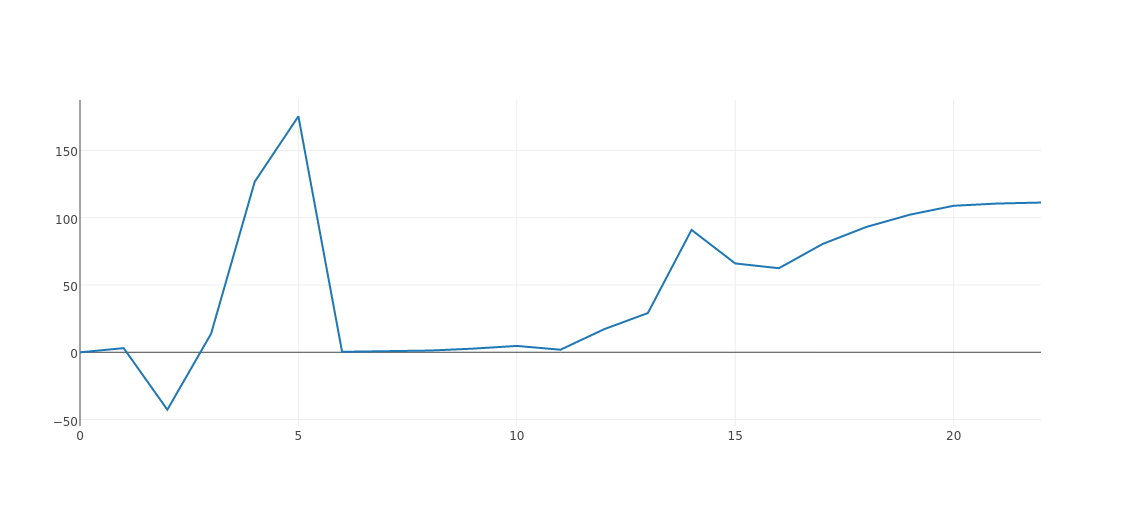
\includegraphics[scale=0.4]{./graphs/ppcap_ext.png}
		\caption{График зависимости Rpp(k), Mb/sec (процессы на разных узлах сети)}
		\captionsetup{labelformat=empty}
	\end{figure}
	
	\begin{figure}[H]
		\centering
		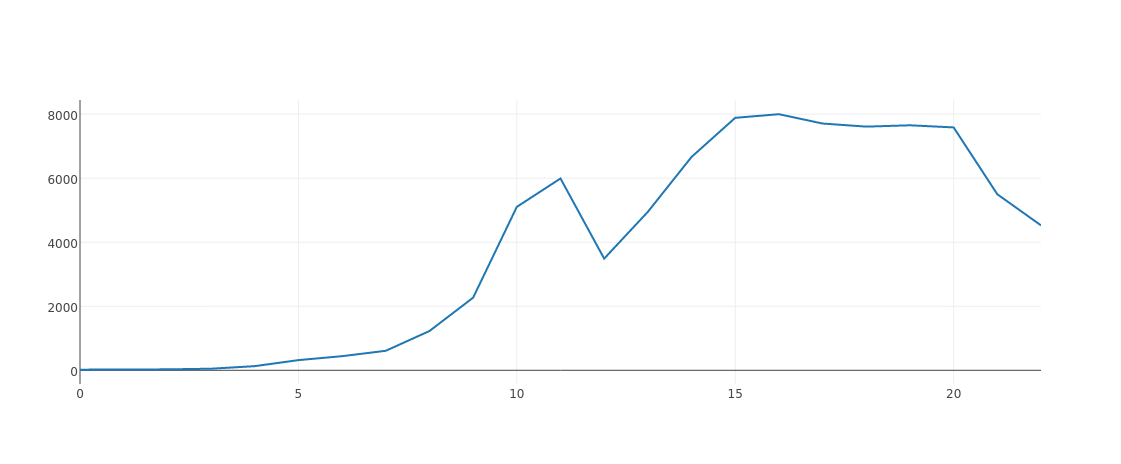
\includegraphics[scale=0.4]{./graphs/dcap_int.png}
		\caption{График зависимости Rd(k), Mb/sec (процессы на одном узле сети)}
		\captionsetup{labelformat=empty}
	\end{figure}
	
	\begin{figure}[H]
		\centering
		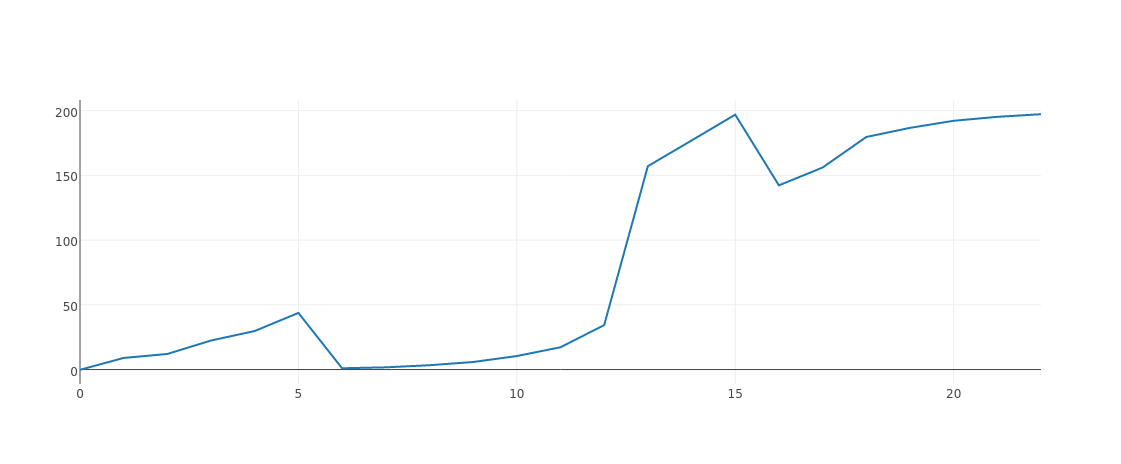
\includegraphics[scale=0.4]{./graphs/dcap_ext.png}
		\caption{График зависимости Rpp(k), Mb/sec (процессы на разных узлах сети)}
		\captionsetup{labelformat=empty}
	\end{figure}
	
	\bigskip
	\qquad Видим, что при запуске процессов на одном узле латентность практически никак не зависит от размера сообщения, в то время как при запуске на разных узлах s выходит на константу при росте k.\\
	\qquad Картины для Rpp и Rd при запуске на одном узле почти идентичны, пропусакная способность приближается к некоторой константе с ростом k, присутствует лишь не очень знаительная разница в скорости. Когда k мало, то есть мала длина посылаемого сообщения, время латентности, которое зависит лишь от числа пересылок, а не от L, начинает играть более существенную роль, и пропускная способность близка к 0. При запуске же на различных узлах графики также схожи, однако у графика Rpp имеется занятный пик при $k=3, 4, 5$. Предположительно он может быть обусловлен совпадением буфера односторонней посылки с размером передаваемого сообщения, что могло существенно ускорить процесс. \\ \bigskip
	
	\qquad Ну и напоследок сравним полученные результаты с соответствующими значениями суперкомпьюера Sequoia:
	\begin{figure}[H]
		\centering
		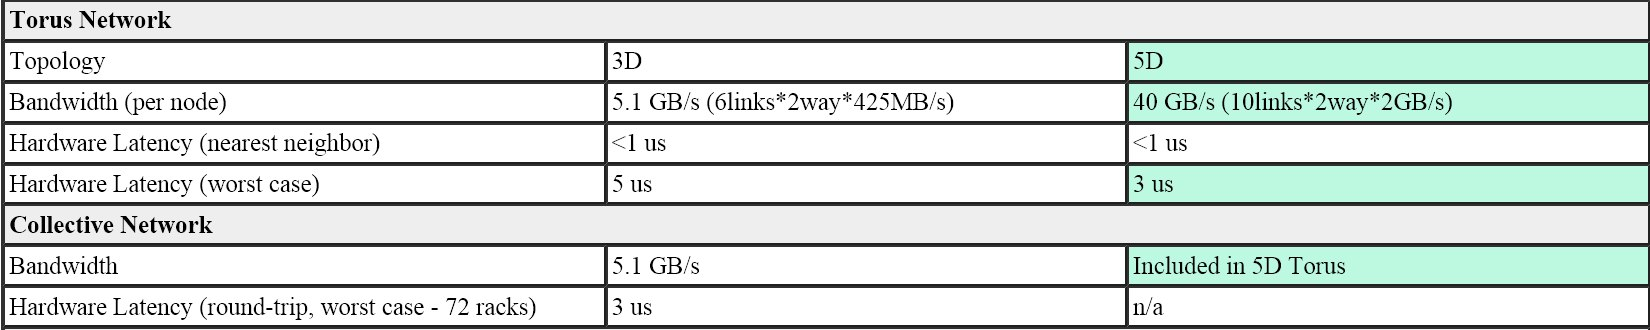
\includegraphics[scale=0.5]{./sequoia.jpg}
		\caption{Показатели Sequoia}
		\captionsetup{labelformat=empty}
	\end{figure}
	
\end{document}